%% Creator: Inkscape inkscape 0.48.4, www.inkscape.org
%% PDF/EPS/PS + LaTeX output extension by Johan Engelen, 2010
%% Accompanies image file 'experimental_setup_small.pdf' (pdf, eps, ps)
%%
%% To include the image in your LaTeX document, write
%%   \input{<filename>.pdf_tex}
%%  instead of
%%   \includegraphics{<filename>.pdf}
%% To scale the image, write
%%   \def\svgwidth{<desired width>}
%%   \input{<filename>.pdf_tex}
%%  instead of
%%   \includegraphics[width=<desired width>]{<filename>.pdf}
%%
%% Images with a different path to the parent latex file can
%% be accessed with the `import' package (which may need to be
%% installed) using
%%   \usepackage{import}
%% in the preamble, and then including the image with
%%   \import{<path to file>}{<filename>.pdf_tex}
%% Alternatively, one can specify
%%   \graphicspath{{<path to file>/}}
%% 
%% For more information, please see info/svg-inkscape on CTAN:
%%   http://tug.ctan.org/tex-archive/info/svg-inkscape
%%
\begingroup%
  \makeatletter%
  \providecommand\color[2][]{%
    \errmessage{(Inkscape) Color is used for the text in Inkscape, but the package 'color.sty' is not loaded}%
    \renewcommand\color[2][]{}%
  }%
  \providecommand\transparent[1]{%
    \errmessage{(Inkscape) Transparency is used (non-zero) for the text in Inkscape, but the package 'transparent.sty' is not loaded}%
    \renewcommand\transparent[1]{}%
  }%
  \providecommand\rotatebox[2]{#2}%
  \ifx\svgwidth\undefined%
    \setlength{\unitlength}{439.83422071bp}%
    \ifx\svgscale\undefined%
      \relax%
    \else%
      \setlength{\unitlength}{\unitlength * \real{\svgscale}}%
    \fi%
  \else%
    \setlength{\unitlength}{\svgwidth}%
  \fi%
  \global\let\svgwidth\undefined%
  \global\let\svgscale\undefined%
  \makeatother%
  \begin{picture}(1,0.50924798)%
    \put(0,0){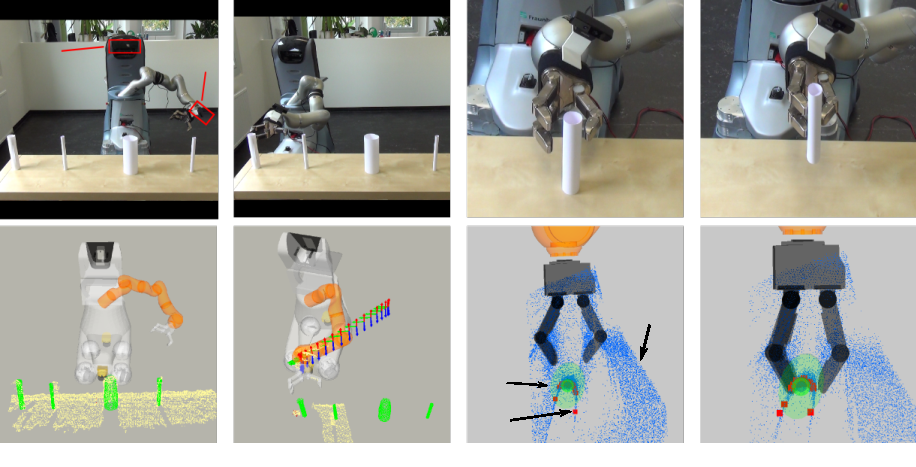
\includegraphics[width=\unitlength]{experimental_setup_small.pdf}}%
    \put(0.04104872,0.44233287){\color[rgb]{0,0,0}\makebox(0,0)[lb]{\smash{\scriptsize{Kinect}}}}%
    \put(0.18372971,0.44356854){\color[rgb]{0,0,0}\makebox(0,0)[lb]{\smash{\scriptsize{Senz3D}}}}%
    \put(0.06296952,0.30312258){\color[rgb]{0,0,0}\makebox(0,0)[lb]{\smash{\scriptsize{$\o$=2cm}}}}%
    \put(0.00 ,0.3049042){\color[rgb]{0,0,0}\makebox(0,0)[lb]{\smash{\scriptsize{$\o$=8cm}}}}%
    \put(0.12743073,0.29969816){\color[rgb]{0,0,0}\makebox(0,0)[lb]{\smash{\scriptsize{$\o$=8cm}}}}%
    \put(0.19114325,0.29981389){\color[rgb]{0,0,0}\makebox(0,0)[lb]{\smash{\scriptsize{$\o$=2cm}}}}%
    \put(0.11772753,0.00025755){\color[rgb]{0,0,0}\makebox(0,0)[lb]{\smash{(a)}}}%
    \put(0.36327459,0.00025755){\color[rgb]{0,0,0}\makebox(0,0)[lb]{\smash{(b)}}}%
    \put(0.62701032,0.00025755){\color[rgb]{0,0,0}\makebox(0,0)[lb]{\smash{(c)}}}%
    \put(0.88165172,0.00025755){\color[rgb]{0,0,0}\makebox(0,0)[lb]{\smash{(d)}}}%
    \put(0.68157634,0.16395559){\color[rgb]{0,0,0}\makebox(0,0)[lb]{\smash{\scriptsize{Point cloud}}}}%
    \put(0.5178783,0.10029525){\color[rgb]{0,0,0}\makebox(0,0)[lb]{\smash{\scriptsize{Uncertainty  ellipse}}}}%
    \put(0.51464349,0.03764591){\color[rgb]{0,0,0}\makebox(0,0)[lb]{\smash{\scriptsize{filtered points for tracking}}}}%
  \end{picture}%
\endgroup%
